\documentclass[../main.tex]{subfiles}
\graphicspath{{\subfix{../images/}}}
\begin{document}

Consider this portion of $W^{(out)}$: 
%Portion of the network picture
\begin{center}
    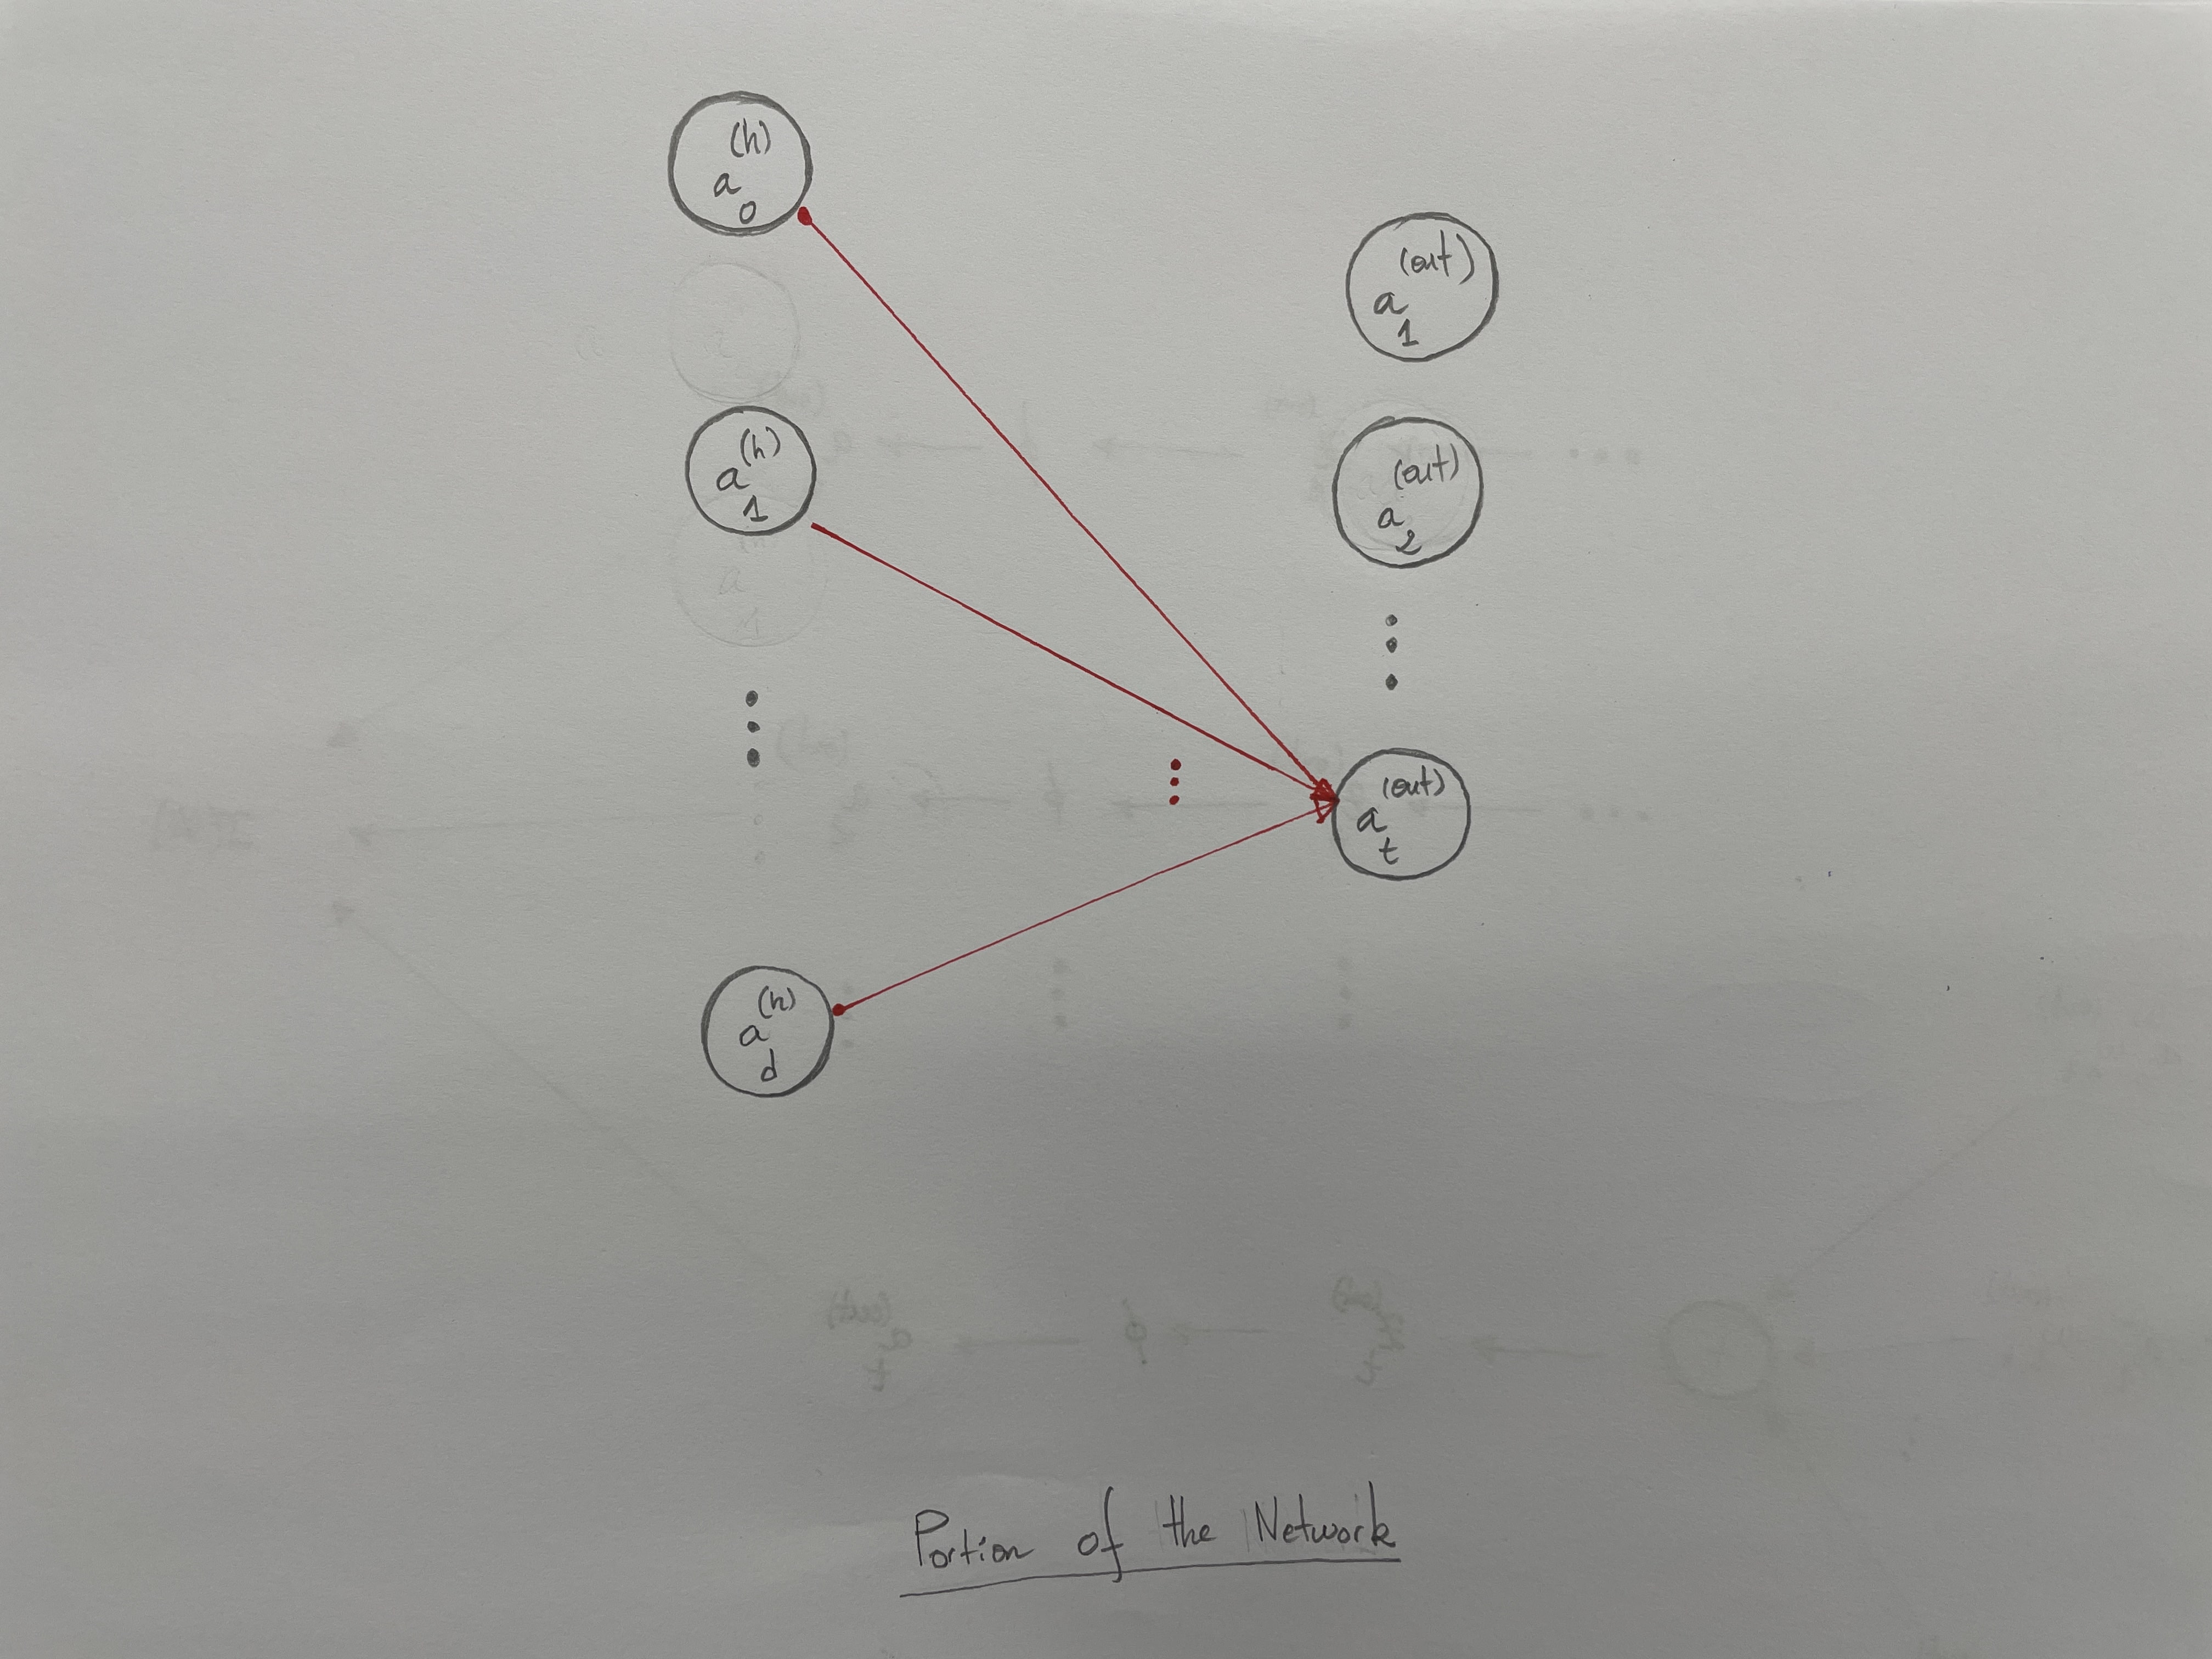
\includegraphics[width = 13cm, height = 9cm]{5.jpg}
\end{center}

\vspace{5mm} %5mm vertical space

The connections $w_{0,t}^{(out)}$, $w_{1,t}^{(out)}$, ..., $w_{d,t}^{(out)}$ are highlighted
in red. Let's look at them in detail...

\vspace{5mm} %5mm vertical space

%Portion of the network picture
\begin{center}
    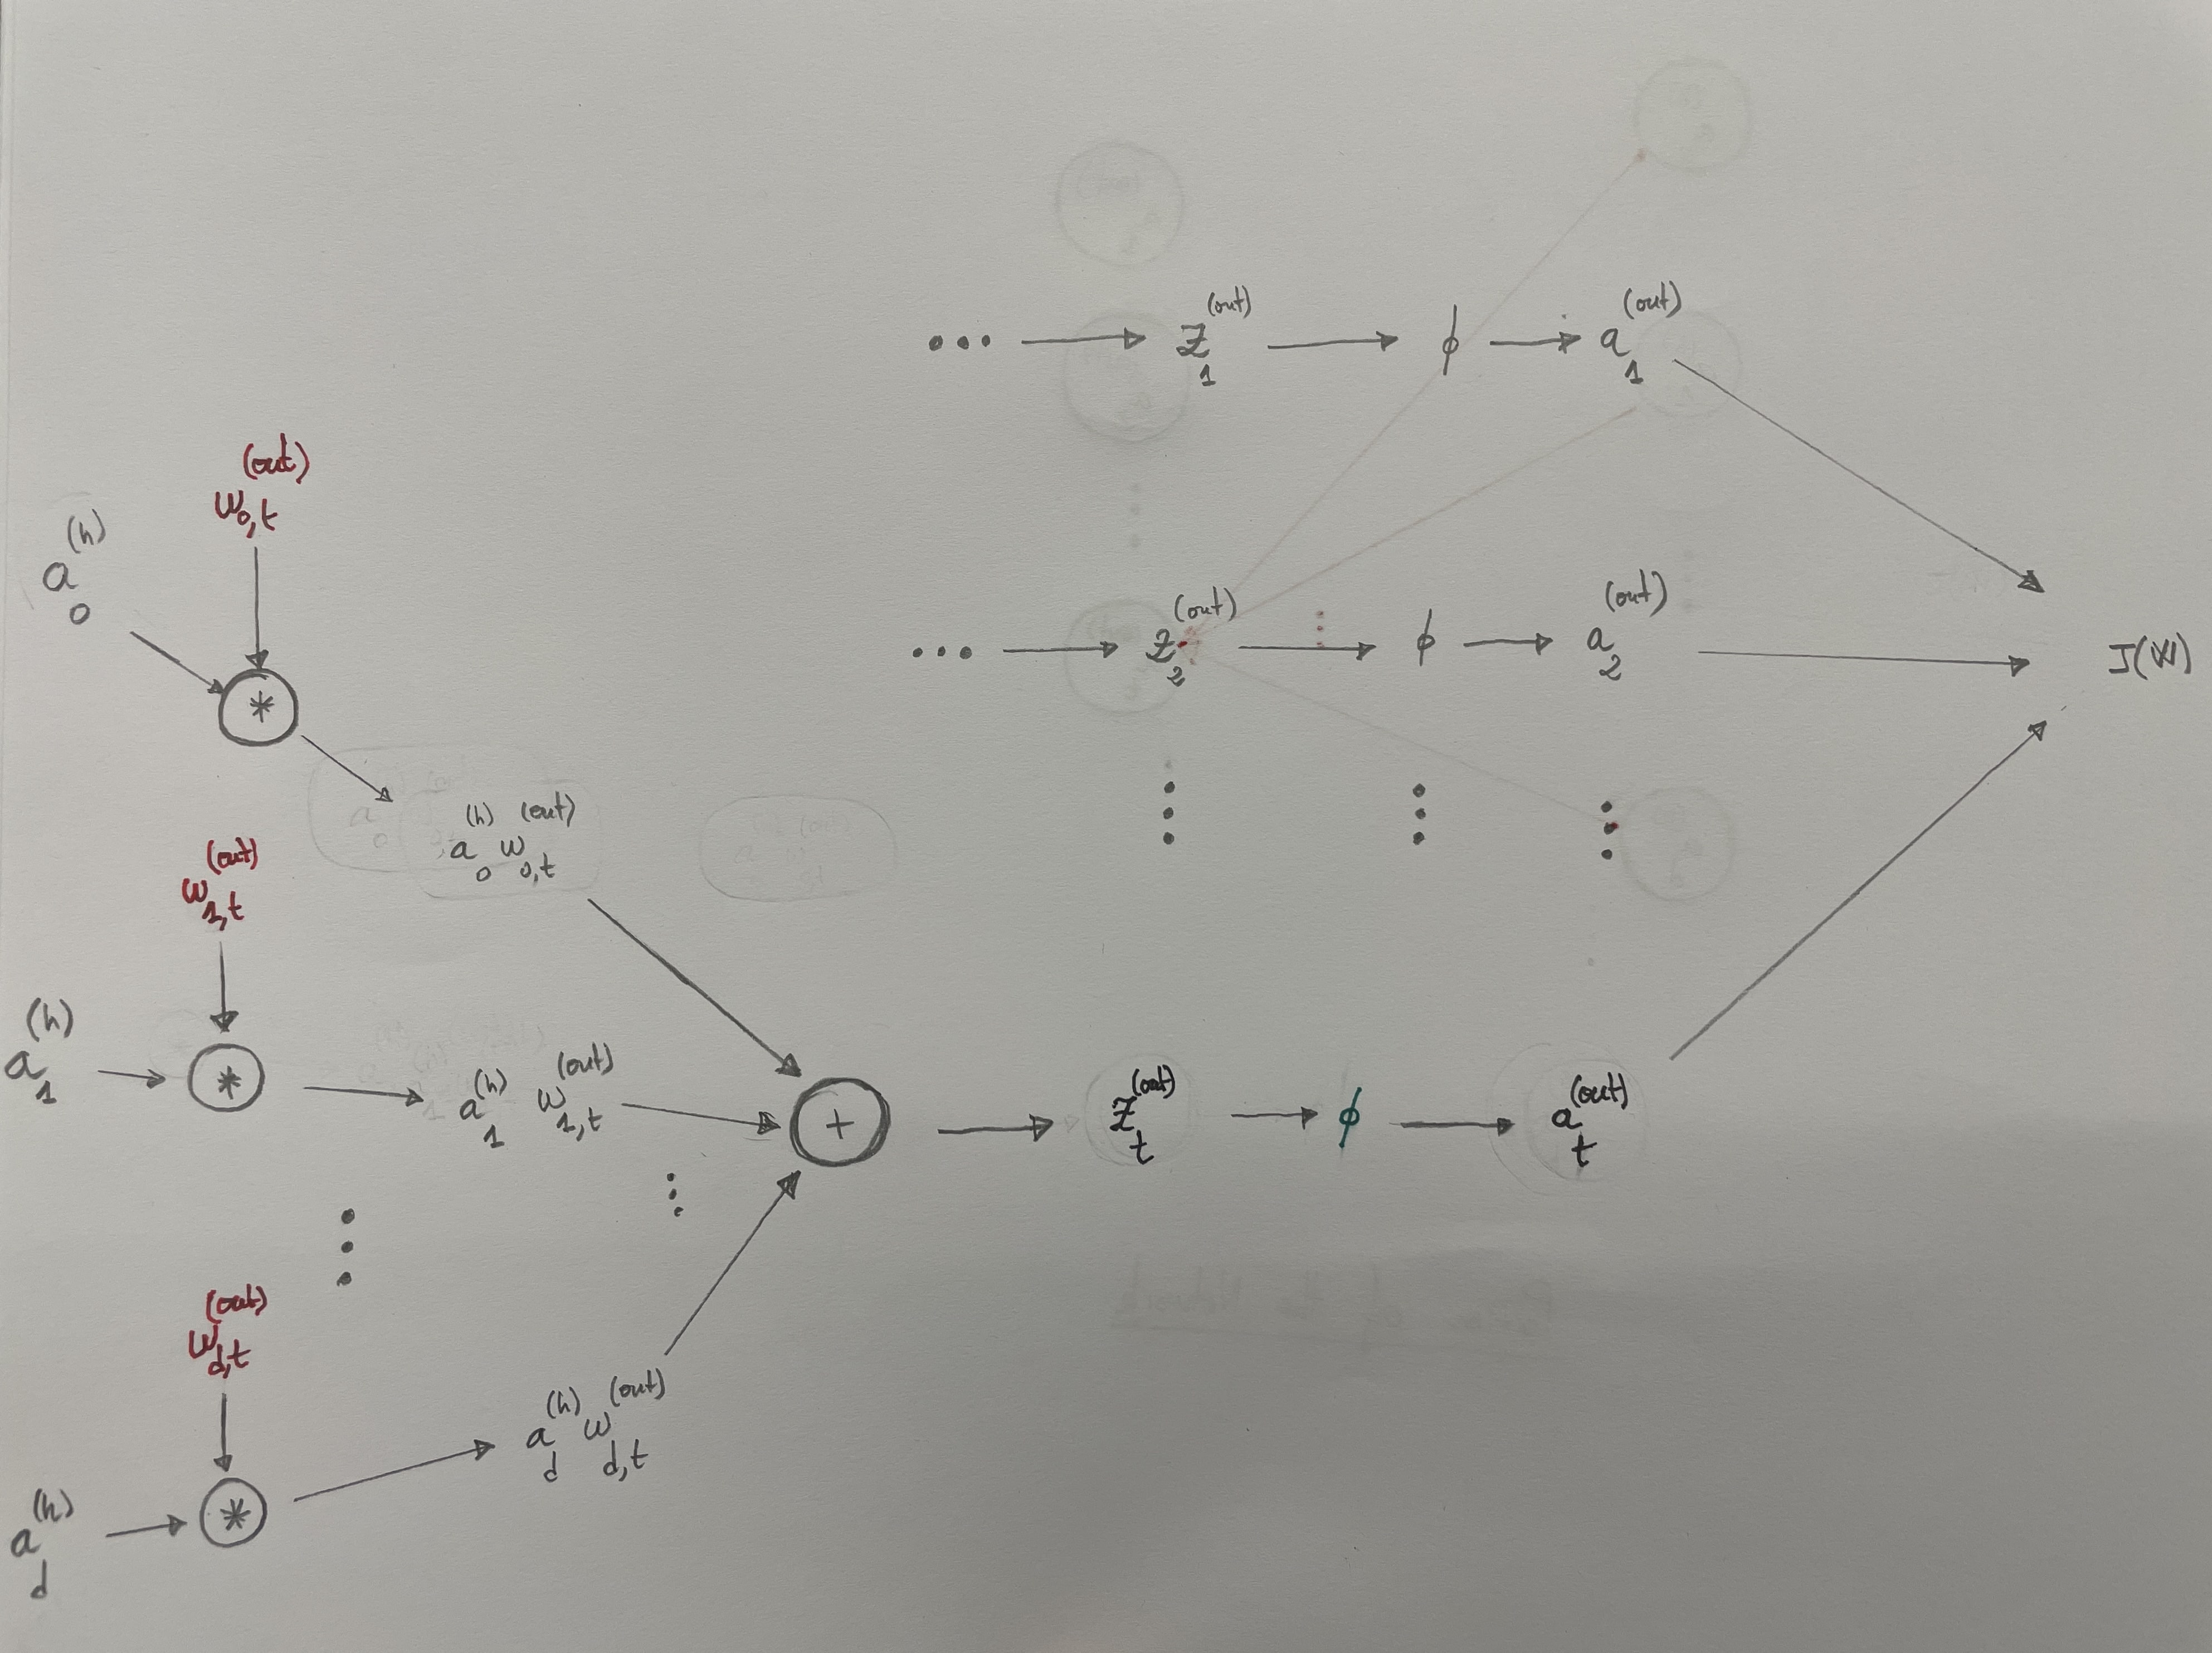
\includegraphics[width = 14cm, height = 9cm]{6.jpg}
\end{center}

\vspace{5mm} %5mm vertical space

On the image above, you are looking at graph representation of the portion we are focusing on. You can see
how the weights \textcolor{red}{$w_{0,t}^{(out)}$}, \textcolor{red}{$w_{1,t}^{(out)}$}, ... 
\textcolor{red}{$w_{d,t}^{(out)}$} get multiplied with the activations of the hidden layer 
and how subsequent operations result in activation value $a_t^{(out)}$ activation unit in the
output layer of our MLP.

\vspace{5mm} %5mm vertical space

To get to the formula Dr. Raschka used, we must \textbf{backpropagate}. In other words,
we must compute the gradient of $J(W)$ w.r.t \emph{all} the weights in $W^{(out)}$. 

\vspace{5mm} %5mm vertical space

Since we focused our attention on $w_{0,t}^{(out)}$, $w_{1,t}^{(out)}$, ... $w_{d,t}^{(out)}$.
Let's manually compute their gradients!

\vspace{5mm} %5mm vertical space

We start at $J(W)$. When we take the partial derivative of the loss w.r.t itself. We get $1$
\[\frac{\partial J(W)}{\partial J(W)} = 1 \]

\vspace{5mm} %5mm vertical space

I continue with $a_{t}^{(out)}$

\[
    \frac{\partial J(W)}{\partial a_{t}^{(out)}} =
    \frac{a_{t}^{(out)} - y_{t}}{a_{t}^{(out)}(1 - a_{t}^{(out)})}
\]

In case you wonder how I came up with this result, I wrote another document about it [LINK IT]

\vspace{5mm} %5mm vertical space

I move on with $z_{t}^{(out)}$

\[
    \frac{\partial J(W)}{\partial z_{t}^{(out)}} =
    \frac{\partial a_{t}^{(out)}}{\partial z_{t}^{(out)}} \times
    \frac{\partial J(W)}{\partial a_{t}^{(out)}} =
    a_{t}^{(out)}(1 - a_{t}^{(out)}) \bullet \frac{\partial J(W)}{\partial a_{t}^{(out)}} =
    a_{t}^{(out)} - y_t
\]

\vspace{5mm} %5mm vertical space

Let's continue with $a_0^{(h)}w_{0,t}^{(out)}$, $a_1^{(h)}w_{1,t}^{(out)}$, ..., $a_d^{(h)}w_{d,t}^{(out)}$

\[
    \frac{\partial J(W)}{\partial a_0^{(h)}w_{0,t}^{(out)}} =
    \frac{\partial J(W)}{\partial a_1^{(h)}w_{1,t}^{(out)}} =
    \dots =
    \frac{\partial J(W)}{\partial a_d^{(h)}w_{d,t}^{(out)}} = 
    a_{t}^{(out)} - y_t
\]

\vspace{5mm} %5mm vertical space

Conveniently, they all have the same gradients. I encourage you to compute the chain rule and see why.

\vspace{5mm} %5mm vertical space

We can now determine the gradient of  $w_{0,t}^{(out)}$, $w_{1,t}^{(out)}$, ... $w_{d,t}^{(out)}$.
I will ignore the bias weight $w_{0,t}^{(out)}$, but will come to later in the document.

\pagebreak

\[
    \frac{\partial J(W)}{\partial w_{1,t}^{(out)}} =
    \frac{\partial a_1^{(h)}w_{1,t}^{(out)}}{\partial w_{1,t}^{(out)}} \times
    \frac{\partial J(W)}{\partial a_1^{(h)}w_{1,t}^{(out)}}  =
    a_1^{(h)}(a_{t}^{(out)} - y_{t})
\]

\[ \vdots \]

\[
    \frac{\partial J(W)}{\partial w_{d,t}^{(out)}} =
    \frac{\partial a_d^{(h)}w_{d,t}^{(out)}}{\partial w_{d,t}^{(out)}} \times
    \frac{\partial J(W)}{\partial a_d^{(h)}w_{d,t}^{(out)}}  =
    a_d^{(h)}(a_{t}^{(out)} - y_{t})
\]

Notice, how $a_{t}^{(out)} - y_{t}$ repeats in the results we found. 
Let's call this expression $\delta_t^{(out)}$.

\vspace{1cm} %1cm vertical space

We now know what the gradients of $w_{0,t}^{(out)}$, $w_{1,t}^{(out)}$, ... $w_{d,t}^{(out)}$ are.
Let's move our attention to another part of the network.

\end{document}